\documentclass[a4j,papersize]{jsbook}

\usepackage[T1]{fontenc} % LaTeXのフォントのエンコーディングをT1にする
\usepackage{textcomp} % TS1
\usepackage[utf8]{inputenc} % ファイルのエンコーディングをUTF8にする
\usepackage{lmodern}

%\usepackage{url}

\usepackage{document} % 自作書式集

\usepackage[dvipdfmx,%
 bookmarks=true,%
 bookmarksnumbered=true,%
 colorlinks=true,%
 setpagesize=false,%
 pdftitle={Javaによる抽象化プログラミング技法},%
 pdfauthor={中鉢欣秀},%
 pdfsubject={教科書},%
 pdfkeywords={Java; Object-Oriented Programing; Framework;}]{hyperref}
\usepackage{pxjahyper}

%%%%%%%%%%%%%%%%%%%%%%%%%%%%%%%%%%%%%%%%%%%%%%%%%%%%%%%%%%%%%%%%%%%%%%%%%%%%%%
% 本文
%%%%%%%%%%%%%%%%%%%%%%%%%%%%%%%%%%%%%%%%%%%%%%%%%%%%%%%%%%%%%%%%%%%%%%%%%%%%%%

%\title{オブジェクト指向フレームワーク原論}d
\title{Javaによる抽象化プログラミング技法}
\author{中鉢 欣秀}
\begin{document}
\maketitle
% \tableofcontents

\chapter*{序}

\begin{abstract}
寿限無寿限無五劫の摺り切れ海砂利水魚の水行末雲来末風来末.食う寝る所に
住む所藪柑子ブラコウジ.パイポパイポパイポのシューリンガングーリンダイ
のポンポコピーのポンポコナーの長久命の長助.
\end{abstract}

\section*{はじめに}

この教科書はオブジェクト指向言語の抽象化機構を最短で理解できることを目
指したものである.

ソフトウェアに関連する技術の移り変わりはとても早い.変わらない知識(普遍的な知識)を身につけることこそ,ソフトウェアのアーキテクトに求められることです.

ソフトウェア・アーキテクチャに関する本質的な知識.

オブジェクト指向の概念に基づくCBD(Component Based Development)を主要なトピックとします.
フレームワークの作り方を学ぶことで,上手な使い方を体得することが目標です.

フレームワークを作れるようになろう 

他人の作ったフレームワークを使って満足するだけ
でよいのか? 

フレームワークを使えるようになろう 

フレームワークの作り方を学ぶことによって、既存
フレームワークをより深く理解することができる 

フレームワーク・プログラミングをとりあげる
理由 

ソフトウェア開発においては、ソフトウェアを部品
化(コンポーネント化)し、部品を再利用すること
で開発効率を上げるための試みが行われてきた。 

フレームワークの構築 

原始的なIPO構造の理解から順をおって、フレーム
ワーク構築までを行ないます。 

オブジェクト指向の最も有用な利用方法の一つとし
てフレームワークとプラグインによるアーキテク
チャ設計を理解しましょう。 

汎用的な技術 

ソフトウェアにおける「構造」とは? 

オブジェクト指向によるフレームワークの設計 

応用的な技術 

Eclipseとプラグインを活用したソフトウェア開発 

実践的なフレームワークのアーキテクチャ 

ソフトウェアの中核的構造をフレームワークとして設計す
る考え方が普及した。 

目的に応じたコンポーネントをフレームワークにプ
ラグインすることで、最も重要で複雑な中核部分の
構造を再利用できるようにする。 

こうすることにより、プログラミングにおける省力化が達
成される。


javaの約束事や決まりごとは「おまじない」または「お約束」と説明するのが
慣例です.
このテキストでは,明確にそれらの解説への参照箇所を示します.

Java言語は初心者向けの言語ではありません.ごく簡単なプログラムであって
もいわゆる「おまじない」がいっぱい出てきます.

Java仕様書

\url{http://docs.oracle.com/javase/specs/jls/se7/jls7-diffs.pdf}

IPOフレームワーク

MVCフレームワーク

\chapter{フレームワークとはなにか}

\begin{abstract}
寿限無寿限無五劫の摺り切れ海砂利水魚の水行末雲来末風来末.食う寝る所に住む所藪柑子ブラコウジ.パイポパイポパイポのシューリンガングーリンダイのポンポコピーのポンポコナーの長久命の長助.
\end{abstract}

\section{フレームワークの定義}
フレームワークの一般的な定義 

1.抽象クラスの集合とそのインスタンス間の相互
作用によって表現された,システムの全体または一
部の再利用可能な設計 

2.開発者がカスタマイズできる,アプリケーショ
ンの骨組み 

 出典) R.ジョンソン,中村宏明,中山裕子,吉田和樹著,
「パターンとフレームワーク」,共立出版 

\section{フレームワークの重要な性質}
ハリウッド・プリンシプル 

映画監督のセリフ 

「Don’t call me, I call you」 

 ハリウッドの役者は,仕事が来るのをひたすら家で待って
いなくてはならない,という例え 

フレームワークは映画監督 

フレームワークの利用者が作成するコンポーネント
は,フレームワークを呼び出すのではなく,フレー
ムワークに呼び出されるのを待つ 

\section{フレームワークに関係する用語}

\begin{figure}
 \begin{center}
  %trim option's parameter order: left bottom right top
  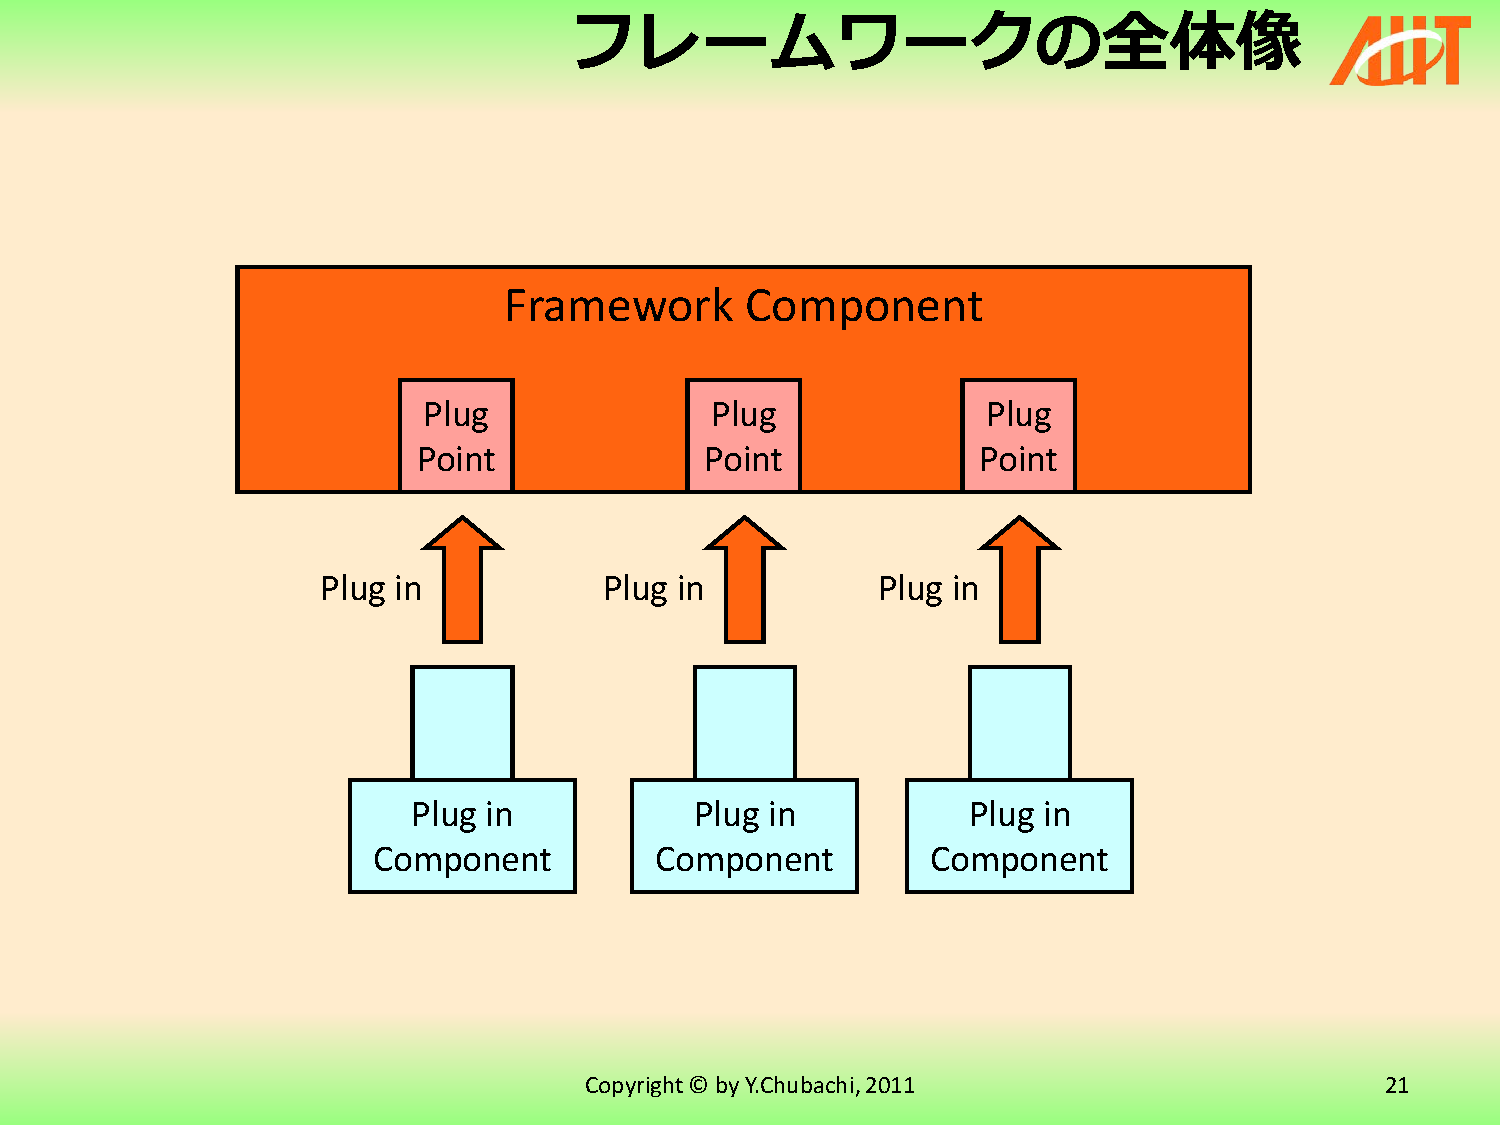
\includegraphics[width=0.8\textwidth, trim=30mm 30mm 35mm
  35mm,clip]{framework.pdf}
  \caption{フレームワークのアーキテクチャ例}
 \end{center}
\end{figure}

\begin{description}
 \item[コンポーネント(component)] 1つまたはそれ以上のクラスからなる,特
	    定の目的を達成するソフトウェア部品.
 \item[フレームワーク・コンポーネント(framework component)] 再利用性の
	    あるロジックをコンポーネントにしたもので,後述のプラグイン
	    コンポーネントと併用することで,様々なアプリケーションに利
	    用できるソフトウェア部品.
 \item[プラグインコンポーネント(Plug-in Component)] フレームワーク・コ
	    ンポーネントに接続することを前提としたコンポーネントで,必
	    要に応じて作成・カスタマイズできる.
 \item[プラグ・ポイント(Plug point)] コンポーネントをフレームワークに
	    プラグインするために,フレームワークが用意する接続点
\end{description}

\section{フレームワークの作り方}
フレームワークの構築へ向けて

段階を追った学習

もととなるプログラムを段階的に進化させる
方針を立て、プログラミング演習で実装する

アーキテクチャの表現と設計

Java言語の各種のOO機能を活用して、フレームワー
クを構築します

クラス/インタフェイス/メソッド/フィールド/パッ
ケージ・・・

モデル(UML)によりアーキテクチャを表現する

\section{リファクタリング・アプローチ}

ボトムアップ・アプローチについて
この授業のスタート地点
 目的の異なる2つのプログラム
フレームワーク構築への道のり
 プログラムの「アーキテクチャ」を捉える
 共通するアーキテクチャを探し出す
 共通化のための方針を立てる
 2つの「上位概念」を考える
 フレームワークを完成させる
リファクタリングとの関連
 このアプローチはリファクタリングの一種でもある

\section{ボトムアップ VS トップダウン}

以上説明したボトムアップのアプローチに対して、トップダウンのアプローチというのもある

最初から抽象度の高いアーキテクチャを「モデル」
として設計し、プログラミングで実装する

ボトムアップを採用する理由

初心者にとって学習曲線が緩やかである

実際の開発の現場でも、トップダウンとボトムアッ
プは併用する

\section{MVCパターン}

% $ pdftk フレームワーク開発特論.pdf cat 29 output MVC.pdf
\begin{figure}
 \begin{center}
  %trim option's parameter order: left bottom right top
  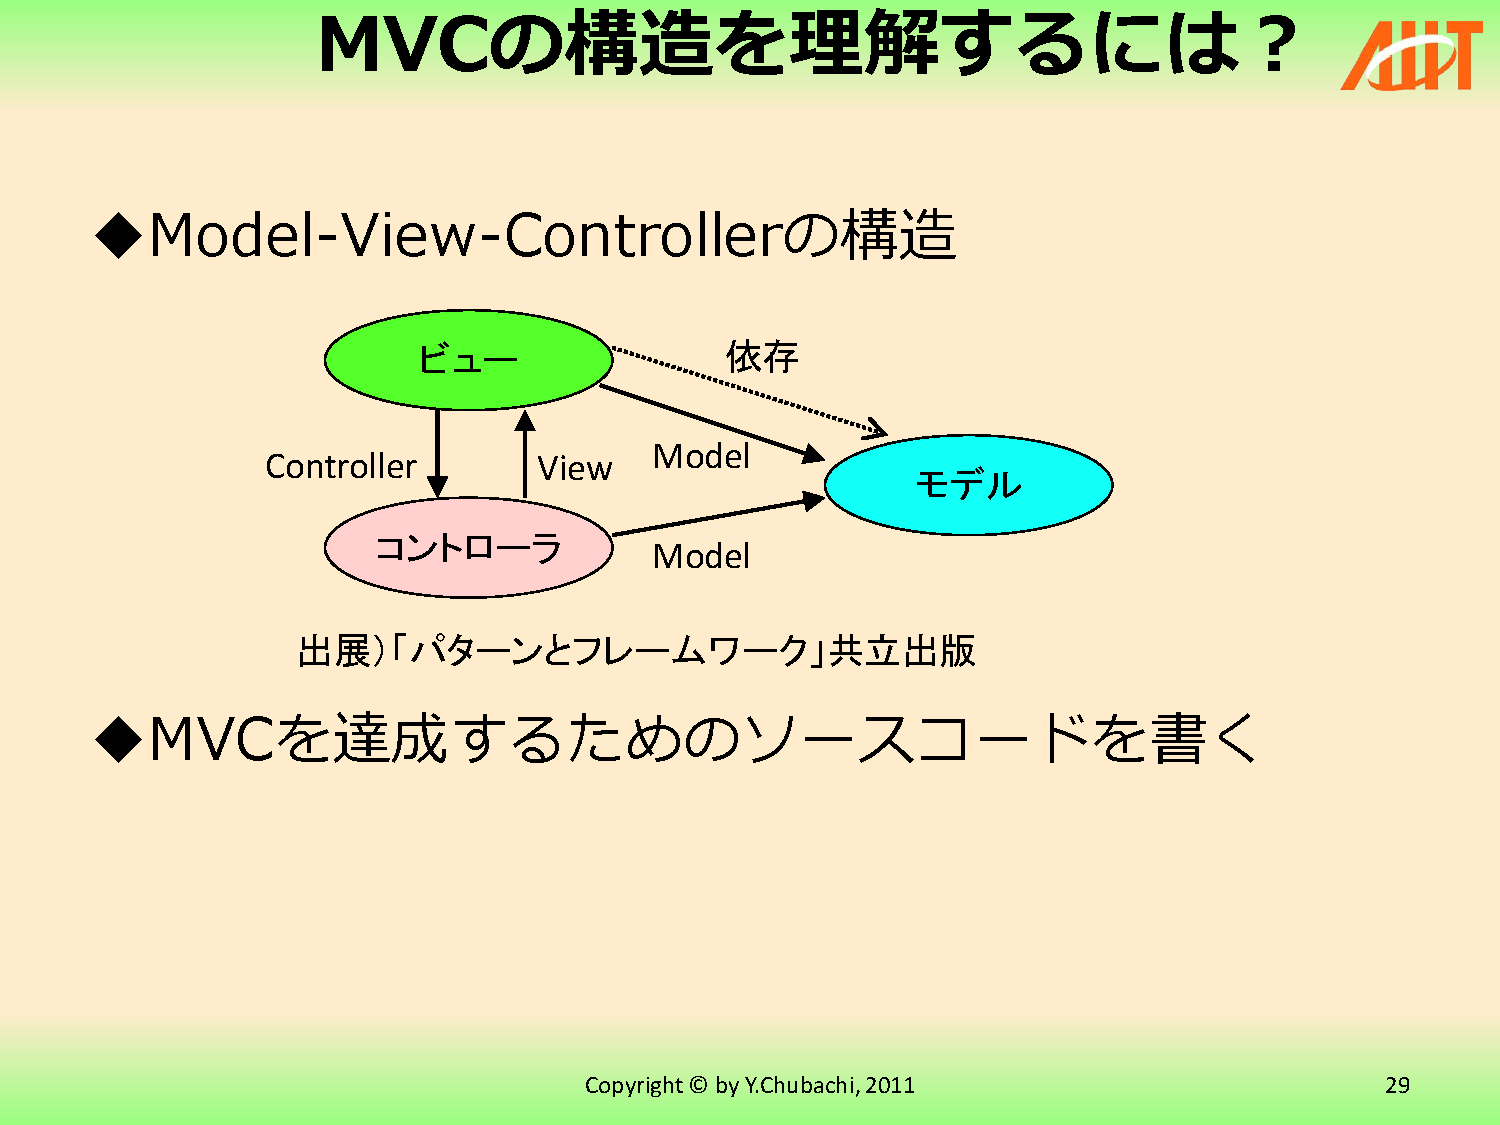
\includegraphics[width=0.8\textwidth, trim=25mm 70mm 60mm 30mm,clip]
   {MVC.pdf}
  \caption{MVC構造(サンプルに合わせて書き直す)}
\end{center}

MVC (Model-View-Controller)の重要性
 主にグラフィカルなインタフェースを備えたソフト
ウェアにおいて,広く一般的に利用するフレーム
ワークである
 近年では、Webアプリケーションの構築にも利用す
る
 ただし、伝統的なMVC構造とは異なっている

MVCは何に使われているのか?

GUIを含むアプリケーションの再利用技術

最初の本格的なオブジェクト指向言語である

SmallTalkで採用

MacintoshのUIでも使用

Microsoft Windowsでも採用

Webアプリケーションに適合するよう変化

MVCの構造を理解するには?

Model-View-Controllerの構造

出展)「パターンとフレームワーク」共立出版
MVCを達成するためのソースコードを書く
 
\end{figure}


\chapter{プログラムのアーキテクチャ}

\begin{abstract}
寿限無寿限無五劫の摺り切れ海砂利水魚の水行末雲来末風来末.食う寝る所に住む所藪柑子ブラコウジ.パイポパイポパイポのシューリンガングーリンダイのポンポコピーのポンポコナーの長久命の長助.
\end{abstract}

\section{全部をmain()に書いた例)}
悪い例

インスタンス化について...

\section{割り算をするプログラム}

次のコードは,Divisionという名前のクラスを定義します.

実際に実行すると,このコードは割り算をして商と余を計算して表示します.

\begin{Verbatim}[commandchars=\\\{\},numbers=left,firstnumber=1,stepnumber=1,frame=single,fontsize=\small]
\PY{k+kn}{package}\PY{+w}{ }\PY{n}{division}\PY{o}{;}

\PY{k+kn}{import}\PY{+w}{ }\PY{n+nn}{java.io.BufferedReader}\PY{o}{;}
\PY{k+kn}{import}\PY{+w}{ }\PY{n+nn}{java.io.InputStreamReader}\PY{o}{;}

\PY{k+kd}{public}\PY{+w}{ }\PY{k+kd}{class}\PY{+w}{ }\PY{n+nc}{Division}\PY{+w}{ }\PY{o}{\PYZob{}}
\PY{+w}{    }\PY{k+kd}{public}\PY{+w}{ }\PY{k+kd}{static}\PY{+w}{ }\PY{k+kt}{void}\PY{+w}{ }\PY{n+nf}{main}\PY{o}{(}\PY{n}{String}\PY{o}{[}\PY{o}{]}\PY{+w}{ }\PY{n}{args}\PY{o}{)}\PY{+w}{ }\PY{k+kd}{throws}\PY{+w}{ }\PY{n}{Exception}\PY{+w}{ }\PY{o}{\PYZob{}}
\PY{+w}{    }\PY{+w}{    }\PY{n}{Division}\PY{+w}{ }\PY{n}{division}\PY{+w}{ }\PY{o}{=}\PY{+w}{ }\PY{k}{new}\PY{+w}{ }\PY{n}{Division}\PY{o}{(}\PY{o}{)}\PY{o}{;}
\PY{+w}{    }\PY{+w}{    }\PY{n}{division}\PY{o}{.}\PY{n+na}{run}\PY{o}{(}\PY{o}{)}\PY{o}{;}
\PY{+w}{    }\PY{o}{\PYZcb{}}
\PY{+w}{    }
\PY{+w}{    }\PY{k+kd}{private}\PY{+w}{ }\PY{k+kt}{void}\PY{+w}{ }\PY{n+nf}{run}\PY{o}{(}\PY{o}{)}\PY{+w}{ }\PY{k+kd}{throws}\PY{+w}{ }\PY{n}{Exception}\PY{+w}{ }\PY{o}{\PYZob{}}
\PY{+w}{    }\PY{+w}{    }\PY{n}{BufferedReader}\PY{+w}{ }\PY{n}{reader}\PY{+w}{ }\PY{o}{=}
\PY{+w}{    }\PY{+w}{    }\PY{+w}{    }\PY{k}{new}\PY{+w}{ }\PY{n+nf}{BufferedReader}\PY{o}{(}\PY{k}{new}\PY{+w}{ }\PY{n}{InputStreamReader}\PY{o}{(}\PY{n}{System}\PY{o}{.}\PY{n+na}{in}\PY{o}{)}\PY{o}{)}\PY{o}{;}
\PY{+w}{    }\PY{+w}{    }\PY{n}{System}\PY{o}{.}\PY{n+na}{out}\PY{o}{.}\PY{n+na}{print}\PY{o}{(}\PY{l+s}{"割られる数を入力してください:"}\PY{o}{)}\PY{o}{;}
\PY{+w}{    }\PY{+w}{    }\PY{n}{String}\PY{+w}{ }\PY{n}{dividendString}\PY{+w}{ }\PY{o}{=}\PY{+w}{ }\PY{n}{reader}\PY{o}{.}\PY{n+na}{readLine}\PY{o}{(}\PY{o}{)}\PY{o}{;}
\PY{+w}{    }\PY{+w}{    }\PY{k+kt}{int}\PY{+w}{ }\PY{n}{dividend}\PY{+w}{ }\PY{o}{=}\PY{+w}{ }\PY{n}{Integer}\PY{o}{.}\PY{n+na}{parseInt}\PY{o}{(}\PY{n}{dividendString}\PY{o}{)}\PY{o}{;}
\PY{+w}{    }\PY{+w}{    }\PY{n}{System}\PY{o}{.}\PY{n+na}{out}\PY{o}{.}\PY{n+na}{print}\PY{o}{(}\PY{l+s}{"割る数を入力してください:"}\PY{o}{)}\PY{o}{;}
\PY{+w}{    }\PY{+w}{    }\PY{n}{String}\PY{+w}{ }\PY{n}{divisorString}\PY{+w}{ }\PY{o}{=}\PY{+w}{ }\PY{n}{reader}\PY{o}{.}\PY{n+na}{readLine}\PY{o}{(}\PY{o}{)}\PY{o}{;}
\PY{+w}{    }\PY{+w}{    }\PY{k+kt}{int}\PY{+w}{ }\PY{n}{divisor}\PY{+w}{ }\PY{o}{=}\PY{+w}{ }\PY{n}{Integer}\PY{o}{.}\PY{n+na}{parseInt}\PY{o}{(}\PY{n}{divisorString}\PY{o}{)}\PY{o}{;}
\PY{+w}{    }\PY{+w}{    }\PY{n}{System}\PY{o}{.}\PY{n+na}{out}\PY{o}{.}\PY{n+na}{print}\PY{o}{(}\PY{l+s}{"商は"}\PY{+w}{ }\PY{o}{+}\PY{+w}{ }\PY{n}{dividend}\PY{+w}{ }\PY{o}{/}\PY{+w}{ }\PY{n}{divisor}
\PY{+w}{    }\PY{+w}{    }\PY{+w}{    }\PY{+w}{    }\PY{o}{+}\PY{+w}{ }\PY{l+s}{"で余は"}\PY{+w}{ }\PY{o}{+}\PY{+w}{ }\PY{n}{dividend}\PY{+w}{ }\PY{o}{\PYZpc{}}\PY{+w}{ }\PY{n}{divisor}\PY{+w}{ }\PY{o}{+}\PY{+w}{ }\PY{l+s}{"です"}\PY{o}{)}\PY{o}{;}
\PY{+w}{    }\PY{o}{\PYZcb{}}
\PY{o}{\PYZcb{}}
\end{Verbatim}


1行目はsquareというパッケージ宣言です(正式は?)\marginpar{パッケージ
については・・・を参照.}.

\section{コメント・ブロック}
それでは,次の例題を考えてみましょう.

\begin{例題}
 Divisionクラスの\texttt{run()}メソッド内のコードを入力・処理・出力のパ
 ターンで分類せよ.
\end{例題}

このクラスをUMLで表現する.

答えは次のとおりです.

\begin{Verbatim}[commandchars=\\\{\},numbers=left,firstnumber=1,stepnumber=1,frame=single,fontsize=\small]
\PY{k+kn}{package}\PY{+w}{ }\PY{n}{division}\PY{o}{;}

\PY{k+kn}{import}\PY{+w}{ }\PY{n+nn}{java.io.BufferedReader}\PY{o}{;}
\PY{k+kn}{import}\PY{+w}{ }\PY{n+nn}{java.io.InputStreamReader}\PY{o}{;}

\PY{k+kd}{public}\PY{+w}{ }\PY{k+kd}{class}\PY{+w}{ }\PY{n+nc}{Division}\PY{+w}{ }\PY{o}{\PYZob{}}
\PY{+w}{    }\PY{k+kd}{public}\PY{+w}{ }\PY{k+kd}{static}\PY{+w}{ }\PY{k+kt}{void}\PY{+w}{ }\PY{n+nf}{main}\PY{o}{(}\PY{n}{String}\PY{o}{[}\PY{o}{]}\PY{+w}{ }\PY{n}{args}\PY{o}{)}\PY{+w}{ }\PY{k+kd}{throws}\PY{+w}{ }\PY{n}{Exception}\PY{+w}{ }\PY{o}{\PYZob{}}
\PY{+w}{    }\PY{+w}{    }\PY{n}{Division}\PY{+w}{ }\PY{n}{division}\PY{+w}{ }\PY{o}{=}\PY{+w}{ }\PY{k}{new}\PY{+w}{ }\PY{n}{Division}\PY{o}{(}\PY{o}{)}\PY{o}{;}
\PY{+w}{    }\PY{+w}{    }\PY{n}{division}\PY{o}{.}\PY{n+na}{run}\PY{o}{(}\PY{o}{)}\PY{o}{;}
\PY{+w}{    }\PY{o}{\PYZcb{}}
\PY{+w}{    }
\PY{+w}{    }\PY{k+kd}{private}\PY{+w}{ }\PY{k+kt}{void}\PY{+w}{ }\PY{n+nf}{run}\PY{o}{(}\PY{o}{)}\PY{+w}{ }\PY{k+kd}{throws}\PY{+w}{ }\PY{n}{Exception}\PY{+w}{ }\PY{o}{\PYZob{}}
\PY{+w}{    }\PY{+w}{    }\PY{c+c1}{//}\PY{+w}{ }\PY{c+c1}{割られる数と割る数を読み込む}
\PY{+w}{    }\PY{+w}{    }\PY{n}{BufferedReader}\PY{+w}{ }\PY{n}{reader}\PY{+w}{ }\PY{o}{=}
\PY{+w}{    }\PY{+w}{    }\PY{+w}{    }\PY{k}{new}\PY{+w}{ }\PY{n+nf}{BufferedReader}\PY{o}{(}\PY{k}{new}\PY{+w}{ }\PY{n}{InputStreamReader}\PY{o}{(}\PY{n}{System}\PY{o}{.}\PY{n+na}{in}\PY{o}{)}\PY{o}{)}\PY{o}{;}
\PY{+w}{    }\PY{+w}{    }\PY{n}{System}\PY{o}{.}\PY{n+na}{out}\PY{o}{.}\PY{n+na}{print}\PY{o}{(}\PY{l+s}{"割られる数を入力してください:"}\PY{o}{)}\PY{o}{;}
\PY{+w}{    }\PY{+w}{    }\PY{n}{String}\PY{+w}{ }\PY{n}{dividendString}\PY{+w}{ }\PY{o}{=}\PY{+w}{ }\PY{n}{reader}\PY{o}{.}\PY{n+na}{readLine}\PY{o}{(}\PY{o}{)}\PY{o}{;}
\PY{+w}{    }\PY{+w}{    }\PY{k+kt}{int}\PY{+w}{ }\PY{n}{dividend}\PY{+w}{ }\PY{o}{=}\PY{+w}{ }\PY{n}{Integer}\PY{o}{.}\PY{n+na}{parseInt}\PY{o}{(}\PY{n}{dividendString}\PY{o}{)}\PY{o}{;}
\PY{+w}{    }\PY{+w}{    }\PY{n}{System}\PY{o}{.}\PY{n+na}{out}\PY{o}{.}\PY{n+na}{print}\PY{o}{(}\PY{l+s}{"割る数を入力してください:"}\PY{o}{)}\PY{o}{;}
\PY{+w}{    }\PY{+w}{    }\PY{n}{String}\PY{+w}{ }\PY{n}{divisorString}\PY{+w}{ }\PY{o}{=}\PY{+w}{ }\PY{n}{reader}\PY{o}{.}\PY{n+na}{readLine}\PY{o}{(}\PY{o}{)}\PY{o}{;}
\PY{+w}{    }\PY{+w}{    }\PY{k+kt}{int}\PY{+w}{ }\PY{n}{divisor}\PY{+w}{ }\PY{o}{=}\PY{+w}{ }\PY{n}{Integer}\PY{o}{.}\PY{n+na}{parseInt}\PY{o}{(}\PY{n}{divisorString}\PY{o}{)}\PY{o}{;}
\PY{+w}{    }\PY{+w}{    }
\PY{+w}{    }\PY{+w}{    }\PY{c+c1}{//}\PY{+w}{ }\PY{c+c1}{商と余を計算する}
\PY{+w}{    }\PY{+w}{    }\PY{k+kt}{int}\PY{+w}{ }\PY{n}{quotient}\PY{+w}{ }\PY{o}{=}\PY{+w}{ }\PY{n}{dividend}\PY{+w}{ }\PY{o}{/}\PY{+w}{ }\PY{n}{divisor}\PY{o}{;}
\PY{+w}{    }\PY{+w}{    }\PY{k+kt}{int}\PY{+w}{ }\PY{n}{remainder}\PY{+w}{ }\PY{o}{=}\PY{+w}{ }\PY{n}{dividend}\PY{+w}{ }\PY{o}{\PYZpc{}}\PY{+w}{ }\PY{n}{divisor}\PY{o}{;}

\PY{+w}{    }\PY{+w}{    }\PY{c+c1}{//}\PY{+w}{ }\PY{c+c1}{割り算の結果を表示する}
\PY{+w}{    }\PY{+w}{    }\PY{n}{System}\PY{o}{.}\PY{n+na}{out}\PY{o}{.}\PY{n+na}{print}\PY{o}{(}\PY{l+s}{"商は"}\PY{+w}{ }\PY{o}{+}\PY{+w}{ }\PY{n}{quotient}\PY{+w}{ }\PY{o}{+}\PY{+w}{ }\PY{l+s}{"で余は"}\PY{+w}{ }\PY{o}{+}\PY{+w}{ }\PY{n}{remainder}\PY{+w}{ }\PY{o}{+}\PY{+w}{ }\PY{l+s}{"です"}\PY{o}{)}\PY{o}{;}
\PY{+w}{    }\PY{o}{\PYZcb{}}
\PY{o}{\PYZcb{}}
\end{Verbatim}


\section{情報を束ねるクラス}
\begin{Verbatim}[commandchars=\\\{\},numbers=left,firstnumber=1,stepnumber=1,frame=single,fontsize=\small]
\PY{k+kn}{package}\PY{+w}{ }\PY{n}{division}\PY{o}{;}

\PY{k+kn}{import}\PY{+w}{ }\PY{n+nn}{java.io.BufferedReader}\PY{o}{;}
\PY{k+kn}{import}\PY{+w}{ }\PY{n+nn}{java.io.InputStreamReader}\PY{o}{;}

\PY{k+kd}{public}\PY{+w}{ }\PY{k+kd}{class}\PY{+w}{ }\PY{n+nc}{Division}\PY{+w}{ }\PY{o}{\PYZob{}}
\PY{+w}{    }\PY{k+kd}{public}\PY{+w}{ }\PY{k+kd}{static}\PY{+w}{ }\PY{k+kt}{void}\PY{+w}{ }\PY{n+nf}{main}\PY{o}{(}\PY{n}{String}\PY{o}{[}\PY{o}{]}\PY{+w}{ }\PY{n}{args}\PY{o}{)}\PY{+w}{ }\PY{k+kd}{throws}\PY{+w}{ }\PY{n}{Exception}\PY{+w}{ }\PY{o}{\PYZob{}}
\PY{+w}{    }\PY{+w}{    }\PY{n}{Division}\PY{+w}{ }\PY{n}{division}\PY{+w}{ }\PY{o}{=}\PY{+w}{ }\PY{k}{new}\PY{+w}{ }\PY{n}{Division}\PY{o}{(}\PY{o}{)}\PY{o}{;}
\PY{+w}{    }\PY{+w}{    }\PY{n}{division}\PY{o}{.}\PY{n+na}{run}\PY{o}{(}\PY{o}{)}\PY{o}{;}
\PY{+w}{    }\PY{o}{\PYZcb{}}
\PY{+w}{    }
\PY{+w}{    }\PY{k+kd}{private}\PY{+w}{ }\PY{k+kt}{void}\PY{+w}{ }\PY{n+nf}{run}\PY{o}{(}\PY{o}{)}\PY{+w}{ }\PY{k+kd}{throws}\PY{+w}{ }\PY{n}{Exception}\PY{+w}{ }\PY{o}{\PYZob{}}
\PY{+w}{    }\PY{+w}{    }\PY{c+c1}{//}\PY{+w}{ }\PY{c+c1}{割られる数と割る数を読み込む}
\PY{+w}{    }\PY{+w}{    }\PY{n}{DividendAndDivisor}\PY{+w}{ }\PY{n}{input}\PY{+w}{ }\PY{o}{=}\PY{+w}{ }\PY{k}{new}\PY{+w}{ }\PY{n}{DividendAndDivisor}\PY{o}{(}\PY{o}{)}\PY{o}{;}
\PY{+w}{    }\PY{+w}{    }\PY{n}{BufferedReader}\PY{+w}{ }\PY{n}{reader}\PY{+w}{ }\PY{o}{=}
\PY{+w}{    }\PY{+w}{    }\PY{+w}{    }\PY{k}{new}\PY{+w}{ }\PY{n+nf}{BufferedReader}\PY{o}{(}\PY{k}{new}\PY{+w}{ }\PY{n}{InputStreamReader}\PY{o}{(}\PY{n}{System}\PY{o}{.}\PY{n+na}{in}\PY{o}{)}\PY{o}{)}\PY{o}{;}
\PY{+w}{    }\PY{+w}{    }\PY{n}{System}\PY{o}{.}\PY{n+na}{out}\PY{o}{.}\PY{n+na}{print}\PY{o}{(}\PY{l+s}{"割られる数を入力してください:"}\PY{o}{)}\PY{o}{;}
\PY{+w}{    }\PY{+w}{    }\PY{n}{String}\PY{+w}{ }\PY{n}{dividendString}\PY{+w}{ }\PY{o}{=}\PY{+w}{ }\PY{n}{reader}\PY{o}{.}\PY{n+na}{readLine}\PY{o}{(}\PY{o}{)}\PY{o}{;}
\PY{+w}{    }\PY{+w}{    }\PY{n}{input}\PY{o}{.}\PY{n+na}{dividend}\PY{+w}{ }\PY{o}{=}\PY{+w}{ }\PY{n}{Integer}\PY{o}{.}\PY{n+na}{parseInt}\PY{o}{(}\PY{n}{dividendString}\PY{o}{)}\PY{o}{;}
\PY{+w}{    }\PY{+w}{    }\PY{n}{System}\PY{o}{.}\PY{n+na}{out}\PY{o}{.}\PY{n+na}{print}\PY{o}{(}\PY{l+s}{"割る数を入力してください:"}\PY{o}{)}\PY{o}{;}
\PY{+w}{    }\PY{+w}{    }\PY{n}{String}\PY{+w}{ }\PY{n}{divisorString}\PY{+w}{ }\PY{o}{=}\PY{+w}{ }\PY{n}{reader}\PY{o}{.}\PY{n+na}{readLine}\PY{o}{(}\PY{o}{)}\PY{o}{;}
\PY{+w}{    }\PY{+w}{    }\PY{n}{input}\PY{o}{.}\PY{n+na}{divisor}\PY{+w}{ }\PY{o}{=}\PY{+w}{ }\PY{n}{Integer}\PY{o}{.}\PY{n+na}{parseInt}\PY{o}{(}\PY{n}{divisorString}\PY{o}{)}\PY{o}{;}
\PY{+w}{    }\PY{+w}{    }
\PY{+w}{    }\PY{+w}{    }\PY{c+c1}{//}\PY{+w}{ }\PY{c+c1}{商と余を計算する}
\PY{+w}{    }\PY{+w}{    }\PY{n}{QuotientAndRemainder}\PY{+w}{ }\PY{n}{output}\PY{+w}{ }\PY{o}{=}\PY{+w}{ }\PY{k}{new}\PY{+w}{ }\PY{n}{QuotientAndRemainder}\PY{o}{(}\PY{o}{)}\PY{o}{;}
\PY{+w}{    }\PY{+w}{    }\PY{n}{output}\PY{o}{.}\PY{n+na}{quotient}\PY{+w}{ }\PY{o}{=}\PY{+w}{ }\PY{n}{input}\PY{o}{.}\PY{n+na}{dividend}\PY{+w}{ }\PY{o}{/}\PY{+w}{ }\PY{n}{input}\PY{o}{.}\PY{n+na}{divisor}\PY{o}{;}
\PY{+w}{    }\PY{+w}{    }\PY{n}{output}\PY{o}{.}\PY{n+na}{remainder}\PY{+w}{ }\PY{o}{=}\PY{+w}{ }\PY{n}{input}\PY{o}{.}\PY{n+na}{dividend}\PY{+w}{ }\PY{o}{\PYZpc{}}\PY{+w}{ }\PY{n}{input}\PY{o}{.}\PY{n+na}{divisor}\PY{o}{;}

\PY{+w}{    }\PY{+w}{    }\PY{c+c1}{//}\PY{+w}{ }\PY{c+c1}{割り算の結果を表示する}
\PY{+w}{    }\PY{+w}{    }\PY{n}{System}\PY{o}{.}\PY{n+na}{out}\PY{o}{.}\PY{n+na}{print}\PY{o}{(}\PY{l+s}{"商は"}\PY{+w}{ }\PY{o}{+}\PY{+w}{ }\PY{n}{output}\PY{o}{.}\PY{n+na}{quotient}
\PY{+w}{    }\PY{+w}{    }\PY{+w}{    }\PY{+w}{    }\PY{o}{+}\PY{+w}{ }\PY{l+s}{"で余は"}\PY{+w}{ }\PY{o}{+}\PY{+w}{ }\PY{n}{output}\PY{o}{.}\PY{n+na}{remainder}\PY{+w}{ }\PY{o}{+}\PY{+w}{ }\PY{l+s}{"です"}\PY{o}{)}\PY{o}{;}
\PY{+w}{    }\PY{o}{\PYZcb{}}
\PY{o}{\PYZcb{}}
\end{Verbatim}


\section{操作を束ねるクラス}
\begin{Verbatim}[commandchars=\\\{\},numbers=left,firstnumber=1,stepnumber=1,frame=single,fontsize=\small]
\PY{k+kn}{package}\PY{+w}{ }\PY{n}{division}\PY{o}{;}

\PY{k+kn}{import}\PY{+w}{ }\PY{n+nn}{java.io.BufferedReader}\PY{o}{;}
\PY{k+kn}{import}\PY{+w}{ }\PY{n+nn}{java.io.IOException}\PY{o}{;}
\PY{k+kn}{import}\PY{+w}{ }\PY{n+nn}{java.io.InputStreamReader}\PY{o}{;}

\PY{k+kd}{public}\PY{+w}{ }\PY{k+kd}{class}\PY{+w}{ }\PY{n+nc}{Division}\PY{+w}{ }\PY{o}{\PYZob{}}
\PY{+w}{    }\PY{k+kd}{public}\PY{+w}{ }\PY{k+kd}{static}\PY{+w}{ }\PY{k+kt}{void}\PY{+w}{ }\PY{n+nf}{main}\PY{o}{(}\PY{n}{String}\PY{o}{[}\PY{o}{]}\PY{+w}{ }\PY{n}{args}\PY{o}{)}\PY{+w}{ }\PY{k+kd}{throws}\PY{+w}{ }\PY{n}{Exception}\PY{+w}{ }\PY{o}{\PYZob{}}
\PY{+w}{    }\PY{+w}{    }\PY{n}{Division}\PY{+w}{ }\PY{n}{division}\PY{+w}{ }\PY{o}{=}\PY{+w}{ }\PY{k}{new}\PY{+w}{ }\PY{n}{Division}\PY{o}{(}\PY{o}{)}\PY{o}{;}
\PY{+w}{    }\PY{+w}{    }\PY{n}{division}\PY{o}{.}\PY{n+na}{run}\PY{o}{(}\PY{o}{)}\PY{o}{;}
\PY{+w}{    }\PY{o}{\PYZcb{}}
\PY{+w}{    }
\PY{+w}{    }\PY{k+kd}{private}\PY{+w}{ }\PY{k+kt}{void}\PY{+w}{ }\PY{n+nf}{run}\PY{o}{(}\PY{o}{)}\PY{+w}{ }\PY{k+kd}{throws}\PY{+w}{ }\PY{n}{Exception}\PY{+w}{ }\PY{o}{\PYZob{}}
\PY{+w}{    }\PY{+w}{    }\PY{c+c1}{//}\PY{+w}{ }\PY{c+c1}{割られる数と割る数を読み込む}
\PY{+w}{    }\PY{+w}{    }\PY{n}{DividendAndDivisor}\PY{+w}{ }\PY{n}{input}\PY{+w}{ }\PY{o}{=}\PY{+w}{ }\PY{n}{input}\PY{o}{(}\PY{o}{)}\PY{o}{;}
\PY{+w}{    }\PY{+w}{    }\PY{c+c1}{//}\PY{+w}{ }\PY{c+c1}{商と余を計算する}
\PY{+w}{    }\PY{+w}{    }\PY{n}{QuotientAndRemainder}\PY{+w}{ }\PY{n}{output}\PY{+w}{ }\PY{o}{=}\PY{+w}{ }\PY{n}{process}\PY{o}{(}\PY{n}{input}\PY{o}{)}\PY{o}{;}
\PY{+w}{    }\PY{+w}{    }\PY{c+c1}{//}\PY{+w}{ }\PY{c+c1}{割り算の結果を表示する}
\PY{+w}{    }\PY{+w}{    }\PY{n}{output}\PY{o}{(}\PY{n}{output}\PY{o}{)}\PY{o}{;}
\PY{+w}{    }\PY{o}{\PYZcb{}}

\PY{+w}{    }\PY{k+kd}{private}\PY{+w}{ }\PY{n}{DividendAndDivisor}\PY{+w}{ }\PY{n+nf}{input}\PY{o}{(}\PY{o}{)}\PY{+w}{ }\PY{k+kd}{throws}\PY{+w}{ }\PY{n}{IOException}\PY{+w}{ }\PY{o}{\PYZob{}}
\PY{+w}{    }\PY{+w}{    }\PY{n}{DividendAndDivisor}\PY{+w}{ }\PY{n}{input}\PY{+w}{ }\PY{o}{=}\PY{+w}{ }\PY{k}{new}\PY{+w}{ }\PY{n}{DividendAndDivisor}\PY{o}{(}\PY{o}{)}\PY{o}{;}
\PY{+w}{    }\PY{+w}{    }\PY{n}{BufferedReader}\PY{+w}{ }\PY{n}{reader}\PY{+w}{ }\PY{o}{=}
\PY{+w}{    }\PY{+w}{    }\PY{+w}{    }\PY{k}{new}\PY{+w}{ }\PY{n+nf}{BufferedReader}\PY{o}{(}\PY{k}{new}\PY{+w}{ }\PY{n}{InputStreamReader}\PY{o}{(}\PY{n}{System}\PY{o}{.}\PY{n+na}{in}\PY{o}{)}\PY{o}{)}\PY{o}{;}
\PY{+w}{    }\PY{+w}{    }\PY{n}{System}\PY{o}{.}\PY{n+na}{out}\PY{o}{.}\PY{n+na}{print}\PY{o}{(}\PY{l+s}{"割られる数を入力してください:"}\PY{o}{)}\PY{o}{;}
\PY{+w}{    }\PY{+w}{    }\PY{n}{String}\PY{+w}{ }\PY{n}{dividendString}\PY{+w}{ }\PY{o}{=}\PY{+w}{ }\PY{n}{reader}\PY{o}{.}\PY{n+na}{readLine}\PY{o}{(}\PY{o}{)}\PY{o}{;}
\PY{+w}{    }\PY{+w}{    }\PY{n}{input}\PY{o}{.}\PY{n+na}{dividend}\PY{+w}{ }\PY{o}{=}\PY{+w}{ }\PY{n}{Integer}\PY{o}{.}\PY{n+na}{parseInt}\PY{o}{(}\PY{n}{dividendString}\PY{o}{)}\PY{o}{;}
\PY{+w}{    }\PY{+w}{    }\PY{n}{System}\PY{o}{.}\PY{n+na}{out}\PY{o}{.}\PY{n+na}{print}\PY{o}{(}\PY{l+s}{"割る数を入力してください:"}\PY{o}{)}\PY{o}{;}
\PY{+w}{    }\PY{+w}{    }\PY{n}{String}\PY{+w}{ }\PY{n}{divisorString}\PY{+w}{ }\PY{o}{=}\PY{+w}{ }\PY{n}{reader}\PY{o}{.}\PY{n+na}{readLine}\PY{o}{(}\PY{o}{)}\PY{o}{;}
\PY{+w}{    }\PY{+w}{    }\PY{n}{input}\PY{o}{.}\PY{n+na}{divisor}\PY{+w}{ }\PY{o}{=}\PY{+w}{ }\PY{n}{Integer}\PY{o}{.}\PY{n+na}{parseInt}\PY{o}{(}\PY{n}{divisorString}\PY{o}{)}\PY{o}{;}
\PY{+w}{    }\PY{+w}{    }\PY{k}{return}\PY{+w}{ }\PY{n}{input}\PY{o}{;}
\PY{+w}{    }\PY{o}{\PYZcb{}}

\PY{+w}{    }\PY{k+kd}{private}\PY{+w}{ }\PY{n}{QuotientAndRemainder}\PY{+w}{ }\PY{n+nf}{process}\PY{o}{(}\PY{n}{DividendAndDivisor}\PY{+w}{ }\PY{n}{input}\PY{o}{)}\PY{+w}{ }\PY{o}{\PYZob{}}
\PY{+w}{    }\PY{+w}{    }\PY{n}{QuotientAndRemainder}\PY{+w}{ }\PY{n}{output}\PY{+w}{ }\PY{o}{=}\PY{+w}{ }\PY{k}{new}\PY{+w}{ }\PY{n}{QuotientAndRemainder}\PY{o}{(}\PY{o}{)}\PY{o}{;}
\PY{+w}{    }\PY{+w}{    }\PY{n}{output}\PY{o}{.}\PY{n+na}{quotient}\PY{+w}{ }\PY{o}{=}\PY{+w}{ }\PY{n}{input}\PY{o}{.}\PY{n+na}{dividend}\PY{+w}{ }\PY{o}{/}\PY{+w}{ }\PY{n}{input}\PY{o}{.}\PY{n+na}{divisor}\PY{o}{;}
\PY{+w}{    }\PY{+w}{    }\PY{n}{output}\PY{o}{.}\PY{n+na}{remainder}\PY{+w}{ }\PY{o}{=}\PY{+w}{ }\PY{n}{input}\PY{o}{.}\PY{n+na}{dividend}\PY{+w}{ }\PY{o}{\PYZpc{}}\PY{+w}{ }\PY{n}{input}\PY{o}{.}\PY{n+na}{divisor}\PY{o}{;}
\PY{+w}{    }\PY{+w}{    }\PY{k}{return}\PY{+w}{ }\PY{n}{output}\PY{o}{;}
\PY{+w}{    }\PY{o}{\PYZcb{}}

\PY{+w}{    }\PY{k+kd}{private}\PY{+w}{ }\PY{k+kt}{void}\PY{+w}{ }\PY{n+nf}{output}\PY{o}{(}\PY{n}{QuotientAndRemainder}\PY{+w}{ }\PY{n}{output}\PY{o}{)}\PY{+w}{ }\PY{o}{\PYZob{}}
\PY{+w}{    }\PY{+w}{    }\PY{n}{System}\PY{o}{.}\PY{n+na}{out}\PY{o}{.}\PY{n+na}{print}\PY{o}{(}\PY{l+s}{"商は"}\PY{+w}{ }\PY{o}{+}\PY{+w}{ }\PY{n}{output}\PY{o}{.}\PY{n+na}{quotient}\PY{+w}{ }\PY{o}{+}\PY{+w}{ }\PY{l+s}{"で余は"}\PY{+w}{ }\PY{o}{+}\PY{+w}{ }\PY{n}{output}\PY{o}{.}\PY{n+na}{remainder}\PY{+w}{ }\PY{o}{+}\PY{+w}{ }\PY{l+s}{"です"}\PY{o}{)}\PY{o}{;}
\PY{+w}{    }\PY{o}{\PYZcb{}}
\PY{o}{\PYZcb{}}
\end{Verbatim}


\section{Interfaceによる抽象化}
\begin{Verbatim}[commandchars=\\\{\},numbers=left,firstnumber=1,stepnumber=1,frame=single,fontsize=\small]
\PY{k+kn}{package}\PY{+w}{ }\PY{n}{division}\PY{o}{;}
\PY{k+kn}{import}\PY{+w}{ }\PY{n+nn}{java.io.BufferedReader}\PY{o}{;}
\PY{k+kn}{import}\PY{+w}{ }\PY{n+nn}{java.io.IOException}\PY{o}{;}
\PY{k+kn}{import}\PY{+w}{ }\PY{n+nn}{java.io.InputStreamReader}\PY{o}{;}

\PY{k+kn}{import}\PY{+w}{ }\PY{n+nn}{framework.Input}\PY{o}{;}
\PY{k+kn}{import}\PY{+w}{ }\PY{n+nn}{framework.Output}\PY{o}{;}


\PY{k+kd}{public}\PY{+w}{ }\PY{k+kd}{class}\PY{+w}{ }\PY{n+nc}{Division}\PY{+w}{ }\PY{o}{\PYZob{}}
\PY{+w}{    }\PY{k+kd}{public}\PY{+w}{ }\PY{k+kd}{static}\PY{+w}{ }\PY{k+kt}{void}\PY{+w}{ }\PY{n+nf}{main}\PY{o}{(}\PY{n}{String}\PY{o}{[}\PY{o}{]}\PY{+w}{ }\PY{n}{args}\PY{o}{)}\PY{+w}{ }\PY{k+kd}{throws}\PY{+w}{ }\PY{n}{Exception}\PY{+w}{ }\PY{o}{\PYZob{}}
\PY{+w}{    }\PY{+w}{    }\PY{n}{Division}\PY{+w}{ }\PY{n}{division}\PY{+w}{ }\PY{o}{=}\PY{+w}{ }\PY{k}{new}\PY{+w}{ }\PY{n}{Division}\PY{o}{(}\PY{o}{)}\PY{o}{;}
\PY{+w}{    }\PY{+w}{    }\PY{n}{division}\PY{o}{.}\PY{n+na}{run}\PY{o}{(}\PY{o}{)}\PY{o}{;}
\PY{+w}{    }\PY{o}{\PYZcb{}}
\PY{+w}{    }
\PY{+w}{    }
\PY{+w}{    }\PY{k+kd}{private}\PY{+w}{ }\PY{k+kt}{void}\PY{+w}{ }\PY{n+nf}{run}\PY{o}{(}\PY{o}{)}\PY{+w}{ }\PY{k+kd}{throws}\PY{+w}{ }\PY{n}{Exception}\PY{+w}{ }\PY{o}{\PYZob{}}
\PY{+w}{    }\PY{+w}{    }\PY{n}{Input}\PY{+w}{ }\PY{n}{input}\PY{+w}{ }\PY{o}{=}\PY{+w}{ }\PY{n}{input}\PY{o}{(}\PY{o}{)}\PY{o}{;}
\PY{+w}{    }\PY{+w}{    }\PY{n}{Output}\PY{+w}{ }\PY{n}{output}\PY{+w}{ }\PY{o}{=}\PY{+w}{ }\PY{n}{process}\PY{o}{(}\PY{n}{input}\PY{o}{)}\PY{o}{;}
\PY{+w}{    }\PY{+w}{    }\PY{n}{output}\PY{o}{(}\PY{n}{output}\PY{o}{)}\PY{o}{;}
\PY{+w}{    }\PY{o}{\PYZcb{}}

\PY{+w}{    }\PY{c+c1}{//}\PY{+w}{ }\PY{c+c1}{割られる数と割る数を読み込む}
\PY{+w}{    }\PY{k+kd}{private}\PY{+w}{ }\PY{n}{Input}\PY{+w}{ }\PY{n+nf}{input}\PY{o}{(}\PY{o}{)}\PY{+w}{ }\PY{k+kd}{throws}\PY{+w}{ }\PY{n}{IOException}\PY{+w}{ }\PY{o}{\PYZob{}}
\PY{+w}{    }\PY{+w}{    }\PY{n}{DividendAndDivisor}\PY{+w}{ }\PY{n}{input}\PY{+w}{ }\PY{o}{=}\PY{+w}{ }\PY{k}{new}\PY{+w}{ }\PY{n}{DividendAndDivisor}\PY{o}{(}\PY{o}{)}\PY{o}{;}
\PY{+w}{    }\PY{+w}{    }\PY{n}{BufferedReader}\PY{+w}{ }\PY{n}{reader}\PY{+w}{ }\PY{o}{=}
\PY{+w}{    }\PY{+w}{    }\PY{+w}{    }\PY{k}{new}\PY{+w}{ }\PY{n+nf}{BufferedReader}\PY{o}{(}\PY{k}{new}\PY{+w}{ }\PY{n}{InputStreamReader}\PY{o}{(}\PY{n}{System}\PY{o}{.}\PY{n+na}{in}\PY{o}{)}\PY{o}{)}\PY{o}{;}
\PY{+w}{    }\PY{+w}{    }\PY{n}{System}\PY{o}{.}\PY{n+na}{out}\PY{o}{.}\PY{n+na}{print}\PY{o}{(}\PY{l+s}{"割られる数を入力してください:"}\PY{o}{)}\PY{o}{;}
\PY{+w}{    }\PY{+w}{    }\PY{n}{String}\PY{+w}{ }\PY{n}{dividendString}\PY{+w}{ }\PY{o}{=}\PY{+w}{ }\PY{n}{reader}\PY{o}{.}\PY{n+na}{readLine}\PY{o}{(}\PY{o}{)}\PY{o}{;}
\PY{+w}{    }\PY{+w}{    }\PY{n}{input}\PY{o}{.}\PY{n+na}{dividend}\PY{+w}{ }\PY{o}{=}\PY{+w}{ }\PY{n}{Integer}\PY{o}{.}\PY{n+na}{parseInt}\PY{o}{(}\PY{n}{dividendString}\PY{o}{)}\PY{o}{;}
\PY{+w}{    }\PY{+w}{    }\PY{n}{System}\PY{o}{.}\PY{n+na}{out}\PY{o}{.}\PY{n+na}{print}\PY{o}{(}\PY{l+s}{"割る数を入力してください:"}\PY{o}{)}\PY{o}{;}
\PY{+w}{    }\PY{+w}{    }\PY{n}{String}\PY{+w}{ }\PY{n}{divisorString}\PY{+w}{ }\PY{o}{=}\PY{+w}{ }\PY{n}{reader}\PY{o}{.}\PY{n+na}{readLine}\PY{o}{(}\PY{o}{)}\PY{o}{;}
\PY{+w}{    }\PY{+w}{    }\PY{n}{input}\PY{o}{.}\PY{n+na}{divisor}\PY{+w}{ }\PY{o}{=}\PY{+w}{ }\PY{n}{Integer}\PY{o}{.}\PY{n+na}{parseInt}\PY{o}{(}\PY{n}{divisorString}\PY{o}{)}\PY{o}{;}
\PY{+w}{    }\PY{+w}{    }\PY{k}{return}\PY{+w}{ }\PY{n}{input}\PY{o}{;}
\PY{+w}{    }\PY{o}{\PYZcb{}}

\PY{+w}{    }\PY{c+c1}{//}\PY{+w}{ }\PY{c+c1}{商と余を計算する}
\PY{+w}{    }\PY{k+kd}{private}\PY{+w}{ }\PY{n}{Output}\PY{+w}{ }\PY{n+nf}{process}\PY{o}{(}\PY{n}{Input}\PY{+w}{ }\PY{n}{input}\PY{o}{)}\PY{+w}{ }\PY{o}{\PYZob{}}
\PY{+w}{    }\PY{+w}{    }\PY{n}{DividendAndDivisor}\PY{+w}{ }\PY{n}{dad}\PY{+w}{ }\PY{o}{=}\PY{+w}{ }\PY{o}{(}\PY{n}{DividendAndDivisor}\PY{o}{)}\PY{+w}{ }\PY{n}{input}\PY{o}{;}
\PY{+w}{    }\PY{+w}{    }\PY{n}{QuotientAndRemainder}\PY{+w}{ }\PY{n}{output}\PY{+w}{ }\PY{o}{=}\PY{+w}{ }\PY{k}{new}\PY{+w}{ }\PY{n}{QuotientAndRemainder}\PY{o}{(}\PY{o}{)}\PY{o}{;}
\PY{+w}{    }\PY{+w}{    }\PY{n}{output}\PY{o}{.}\PY{n+na}{quotient}\PY{+w}{ }\PY{o}{=}\PY{+w}{ }\PY{n}{dad}\PY{o}{.}\PY{n+na}{dividend}\PY{+w}{ }\PY{o}{/}\PY{+w}{ }\PY{n}{dad}\PY{o}{.}\PY{n+na}{divisor}\PY{o}{;}
\PY{+w}{    }\PY{+w}{    }\PY{n}{output}\PY{o}{.}\PY{n+na}{remainder}\PY{+w}{ }\PY{o}{=}\PY{+w}{ }\PY{n}{dad}\PY{o}{.}\PY{n+na}{dividend}\PY{+w}{ }\PY{o}{\PYZpc{}}\PY{+w}{ }\PY{n}{dad}\PY{o}{.}\PY{n+na}{divisor}\PY{o}{;}
\PY{+w}{    }\PY{+w}{    }\PY{k}{return}\PY{+w}{ }\PY{n}{output}\PY{o}{;}
\PY{+w}{    }\PY{o}{\PYZcb{}}

\PY{+w}{    }\PY{c+c1}{//}\PY{+w}{ }\PY{c+c1}{割り算の結果を表示する}
\PY{+w}{    }\PY{k+kd}{private}\PY{+w}{ }\PY{k+kt}{void}\PY{+w}{ }\PY{n+nf}{output}\PY{o}{(}\PY{n}{Output}\PY{+w}{ }\PY{n}{output}\PY{o}{)}\PY{+w}{ }\PY{o}{\PYZob{}}
\PY{+w}{    }\PY{+w}{    }\PY{n}{QuotientAndRemainder}\PY{+w}{ }\PY{n}{qar}\PY{+w}{ }\PY{o}{=}\PY{+w}{ }\PY{o}{(}\PY{n}{QuotientAndRemainder}\PY{o}{)}\PY{+w}{ }\PY{n}{output}\PY{o}{;}
\PY{+w}{    }\PY{+w}{    }\PY{n}{System}\PY{o}{.}\PY{n+na}{out}\PY{o}{.}\PY{n+na}{print}\PY{o}{(}\PY{l+s}{"商は"}\PY{+w}{ }\PY{o}{+}\PY{+w}{ }\PY{n}{qar}\PY{o}{.}\PY{n+na}{quotient}\PY{+w}{ }\PY{o}{+}\PY{+w}{ }\PY{l+s}{"で余は"}\PY{+w}{ }\PY{o}{+}\PY{+w}{ }\PY{n}{qar}\PY{o}{.}\PY{n+na}{remainder}\PY{+w}{ }\PY{o}{+}\PY{+w}{ }\PY{l+s}{"です"}\PY{o}{)}\PY{o}{;}
\PY{+w}{    }\PY{o}{\PYZcb{}}
\PY{o}{\PYZcb{}}
\end{Verbatim}


\newpage
\section{演習問題}

\begin{演習}
 コメントブロックを用いて,このプログラムを入力・処理・出力に整理しなさ
 い.
 \begin{Verbatim}[commandchars=\\\{\},numbers=left,firstnumber=1,stepnumber=1,frame=single,fontsize=\small]
\PY{k+kn}{package}\PY{+w}{ }\PY{n}{square}\PY{o}{;}

\PY{k+kn}{import}\PY{+w}{ }\PY{n+nn}{java.io.BufferedReader}\PY{o}{;}
\PY{k+kn}{import}\PY{+w}{ }\PY{n+nn}{java.io.InputStreamReader}\PY{o}{;}

\PY{k+kd}{public}\PY{+w}{ }\PY{k+kd}{class}\PY{+w}{ }\PY{n+nc}{Square}\PY{+w}{ }\PY{o}{\PYZob{}}
\PY{+w}{    }\PY{k+kd}{public}\PY{+w}{ }\PY{k+kd}{static}\PY{+w}{ }\PY{k+kt}{void}\PY{+w}{ }\PY{n+nf}{main}\PY{o}{(}\PY{n}{String}\PY{o}{[}\PY{o}{]}\PY{+w}{ }\PY{n}{args}\PY{o}{)}\PY{+w}{ }\PY{k+kd}{throws}\PY{+w}{ }\PY{n}{Exception}\PY{+w}{ }\PY{o}{\PYZob{}}
\PY{+w}{    }\PY{+w}{    }\PY{n}{Square}\PY{+w}{ }\PY{n}{square}\PY{+w}{ }\PY{o}{=}\PY{+w}{ }\PY{k}{new}\PY{+w}{ }\PY{n}{Square}\PY{o}{(}\PY{o}{)}\PY{o}{;}
\PY{+w}{    }\PY{+w}{    }\PY{n}{square}\PY{o}{.}\PY{n+na}{run}\PY{o}{(}\PY{o}{)}\PY{o}{;}
\PY{+w}{    }\PY{o}{\PYZcb{}}

\PY{+w}{    }\PY{k+kd}{private}\PY{+w}{ }\PY{k+kt}{void}\PY{+w}{ }\PY{n+nf}{run}\PY{o}{(}\PY{o}{)}\PY{+w}{ }\PY{k+kd}{throws}\PY{+w}{ }\PY{n}{Exception}\PY{+w}{ }\PY{o}{\PYZob{}}
\PY{+w}{    }\PY{+w}{    }\PY{n}{System}\PY{o}{.}\PY{n+na}{out}\PY{o}{.}\PY{n+na}{print}\PY{o}{(}\PY{l+s}{"自乗を計算する値を入力してください:"}\PY{o}{)}\PY{o}{;}
\PY{+w}{    }\PY{+w}{    }\PY{n}{BufferedReader}\PY{+w}{ }\PY{n}{reader}\PY{+w}{ }\PY{o}{=}
\PY{+w}{    }\PY{+w}{    }\PY{+w}{    }\PY{k}{new}\PY{+w}{ }\PY{n+nf}{BufferedReader}\PY{o}{(}
\PY{+w}{    }\PY{+w}{    }\PY{+w}{    }\PY{+w}{    }\PY{k}{new}\PY{+w}{ }\PY{n+nf}{InputStreamReader}\PY{o}{(}\PY{n}{System}\PY{o}{.}\PY{n+na}{in}\PY{o}{)}\PY{o}{)}\PY{o}{;}
\PY{+w}{    }\PY{+w}{    }\PY{n}{String}\PY{+w}{ }\PY{n}{valueString}\PY{+w}{ }\PY{o}{=}\PY{+w}{ }\PY{n}{reader}\PY{o}{.}\PY{n+na}{readLine}\PY{o}{(}\PY{o}{)}\PY{o}{;}
\PY{+w}{    }\PY{+w}{    }\PY{k+kt}{double}\PY{+w}{ }\PY{n}{value}\PY{+w}{ }\PY{o}{=}\PY{+w}{ }\PY{n}{Double}\PY{o}{.}\PY{n+na}{parseDouble}\PY{o}{(}\PY{n}{valueString}\PY{o}{)}\PY{o}{;}
\PY{+w}{    }\PY{+w}{    }\PY{n}{System}\PY{o}{.}\PY{n+na}{out}\PY{o}{.}\PY{n+na}{println}\PY{o}{(}\PY{l+s}{"計算結果:"}\PY{+w}{ }\PY{o}{+}\PY{+w}{ }\PY{o}{(}\PY{n}{value}\PY{+w}{ }\PY{o}{*}\PY{+w}{ }\PY{n}{value}\PY{o}{)}\PY{o}{)}\PY{o}{;}
\PY{+w}{    }\PY{o}{\PYZcb{}}
\PY{o}{\PYZcb{}}
\end{Verbatim}

\end{演習}

\begin{演習}
 Java言語ではクラスの名前とファイル名を一致させる必要がある.他のオブジェ
 クト指向型言語の場合を調べよ.また,クラス名とファイル名を一致させるこ
 との長所・短所について考察せよ.
\end{演習}
 

\section{パッケージとクラスの可視性}
パッケージは名前空間です.

\chapter{メモ}

\begin{enumerate}
 \item 名前付けと抽象化について(int x = 1; double pi = 3.14)
 \item テストを取り上げるか?
 \item パターンとアーキテクチャについて解説する?
 \item UMLの関連・依存関係について
 \item ライブコーディング
 \item 防衛的プログラミング
 \item interfaceとclassの使い分け
 \item 試行錯誤.あるべき設計を発見するまでに必要だったプロセスvs手
       戻り
\end{enumerate}

\end{document}
